\section{State-Force Estimation: The Discrete Time Kalman Filter}
\label{s:DTKF}
Characterizing terrain mobility conditions in real-time requires knowledge of slip and terrain-vehicle forces. However, using proprioceptive sensors, neither of these can be directly measured and must be estimated using the combination of sensor data and a process model in a filtering algorithm. In this application, a DTKF will be used. The process model will come from the single body model derived in Ch. \ref{ch:RSBD} from eq.'s \ref{eq:RSBD_GBSDX}-\ref{eq:RSBD_WBSDL}
\begin{equation*}
    \dot v_x = v_y\dot\theta + \frac{1}{m_T}\Big(F_R + F_L - R_R - R_L - R_{SD} \Big)
\end{equation*}
\begin{equation*}
    \dot v_y = -v_x\dot\theta + \frac{1}{m_T}\Big(R_{lLF} + R_{lLR} + R_{lRF} + R_{lRR} \Big)
\end{equation*}
\begin{equation*}
    \ddot\theta = \frac{1}{J_T} \Bigg( \frac{b}{2}F_R - \frac{b}{2}F_L - \frac{b}{2}R_R + \frac{b}{2}R_L + \frac{l}{4}R_{lLF} - \frac{l}{4}R_{lLR} + \frac{l}{4}R_{lRF} - \frac{l}{4}R_{lRR} \Bigg)
\end{equation*}
\begin{equation*}
    \ddot\varphi_R = \frac{1}{J_S}\Big(\tau_R - F_Rr - \zeta\dot\varphi_R\Big)
\end{equation*}
\begin{equation*}
   \ddot\varphi_L = \frac{1}{J_S}\Big(\tau_L - F_Lr - \zeta\dot\varphi_L\Big)
\end{equation*}
This model will be modified so that only longitudinal trajectories are considered. This is done not only because it simplifies the process model but also because any attempt to turn will certainly immobilize a tracked vehicle under load. To do this, eq.'s for $\dot v_y$ and and $\ddot\theta$ are omitted, the cross product term $v_y\dot\theta$ is removed from the $\dot v_x$ equation, and the equations for bother driver speeds $\ddot\varphi_L$ and $\ddot\varphi_R$ are combined into a single equation. This yields the following two equations with definitions for the new variables of net traction $F_{net}$ and the resistance torque at the driver $\tau_{res}$
\begin{equation}
    \label{eq:DTKF_GBSD1}
    \dot v_T = \frac{F_{net}-DB}{m_T}
\end{equation}
\begin{equation}
    \label{eq:DTKF_WBSD}
    \ddot \varphi = \frac{\tau - \tau_{res}}{J_S}
\end{equation}
\begin{equation}
    F_{net} \equiv F_R + F_L - R_R - R_L
\end{equation}
\begin{equation}
    \tau_{res} \equiv F_Rr + \zeta\dot\varphi_R + F_Lr + \zeta\dot\varphi_L
\end{equation}
\begin{equation}
    \tau \equiv \tau_R + \tau_L
\end{equation}
In the DTKF, the forces and torque $F_{net}$, $DB$, and $\tau_{res}$ will be considered as part of the state $\mathbf{x}$ to be estimated. In order to make it possible for these force and torque estimates to update, a second order random walk model is used whose form is given by
\begin{equation}
    \begin{bmatrix} \dot{\hat{F}} \\ \ddot{\hat{F}} \end{bmatrix} = \begin{bmatrix} 0 & 1 \\ 0 & 0 \end{bmatrix} \begin{bmatrix} \hat{F} \\ \dot{\hat{F}} \end{bmatrix}
\end{equation}
where $\hat{F}$ is the estimated force or torque and $\dot{\hat{F}}$ and $\ddot{\hat{F}}$ are its higher order first and second derivatives. The state vector of the DTKF can now be written as
\begin{equation*}
    \mathbf{x} = \begin{bmatrix} v_T & \dot\varphi & F_{net} & \dot{F}_{net} & \tau_{res} & \dot\tau_{res} & DB & \dot{DB} \end{bmatrix}^T
\end{equation*}
Since the process model is linear in the state vector $\mathbf{x}$, the model will be written in a continuous time state space form
\begin{equation}\label{eq:CTSS}
    \dot{\mathbf{x}} = \mathbf{A}\mathbf{x} + \mathbf{B}\mathbf{u}
\end{equation}
\begin{equation}
    \mathbf{A} = \begin{bmatrix} 0 & 0 & \frac{1}{m_T} & 0 & 0 & 0 & -\frac{1}{m_T} & 0\\
     0 & 0 & 0 & 0 & -\frac{1}{J_S} & 0 & 0 & 0 \\
     0 & 0 & 0 & 1 & 0 & 0 & 0 & 0 \\
     0 & 0 & 0 & 0 & 0 & 0 & 0 & 0\\
     0 & 0 & 0 & 0 & 0 & 1 & 0 & 0\\
     0 & 0 & 0 & 0 & 0 & 0 & 0 & 0 \\
     0 & 0 & 0 & 0 & 0 & 0 & 0 & 1 \\
     0 & 0 & 0 & 0 & 0 & 0 & 0 & 0\end{bmatrix}
\end{equation}
\begin{equation}
    \mathbf{B} = \begin{bmatrix} 0 & 0 \\
     \frac{1}{J_S} & 0 \\
     0 & 0 \\
     0 & 0 \\
     0 & 0 \\
     0 & 0 \\
     0 & 0 \\
     0 & 0 \end{bmatrix}
\end{equation}
\begin{equation}
    \mathbf{u} = \begin{bmatrix} 0 \\ \tau  \end{bmatrix}
\end{equation}
This set of linear, time-invariant, first order differential equations can be discretized into difference equations using a zero order hold assumption for the system input $\mathbf{u}$ where $\mathbf{F}$ and $\mathbf{G}$ are the plant and input matrices \cite{juang2001identification,stengel2012optimal,simon2006optimal}. 
\begin{equation}\label{eq:DT_Model}
    \mathbf{x}_{k} = \mathbf{F}\mathbf{x}_{k-1} + \mathbf{G}\mathbf{u}_{k-1} + \mathbf{w}_{k-1}
\end{equation}
In eq. \ref{eq:DT_Model}, $\mathbf{w} \sim N(\mathbf{0}_{8\times1},\mathbf{Q}_{8\times8})$ is additive gaussian process noise added after discretization of eq. \ref{eq:CTSS} and denotes disturbances that enter linearly into the system equations. This is an assumption of the DTKF that is not true in practice but still yields accurate estimates. This set of difference equations will serve as the process model for the DTKF.

The DTKF also utilizes sensor measurements to make state-force estimates. In this implementation, sensor availability assumes an IMU, GPS, the tractor CAN network, and a load pin. These sensors will utilize measurements of longitudinal tractor acceleration $\dot v_T$, tractor speed $v_T$, driver speed $\dot\varphi$, and the drawbar load $DB$. These make a linear measurement model whose form is given by
\begin{equation}\label{eq:Measurement_Model}
    \mathbf{y}_k = \mathbf{H}\mathbf{x}_k + \mathbf{v}_k
\end{equation}
\begin{equation}
    \mathbf{y}_k = \begin{bmatrix} \dot v_T & v_T & \dot\varphi & DB \end{bmatrix}^T
\end{equation}
\begin{equation}
    \mathbf{H} = \begin{bmatrix} 
     0 & 0 & \frac{1}{m_T} & 0 & 0 & 0 & -\frac{1}{m_T} & 0\\
     1 & 0 & 0 & 0 & 0 & 0 & 0 & 0\\
     0 & 1 & 0 & 0 & 0 & 0 & 0 & 0\\
     0 & 0 & 0 & 0 & 0 & 0 & 1 & 0 \end{bmatrix}
\end{equation}
where $\mathbf{v}_k \sim N(\mathbf{0}_{4\times1},\mathbf{Q}_{4\times4})$ is the measurement noise at time step $k$ whose probability density function is zero-mean Gaussian.

Equations \ref{eq:DT_Model} and \ref{eq:Measurement_Model} consist of linear process and linear measurement models with additive Gaussian process disturbances and sensor noise required for DTKF. This filtering algorithm propagates a Gaussian probability density function (PDF) of the state estimate using a linear process model and combines this estimate with a PDF of the measurement by utilizing the fact the the product of two gaussian functions is another Gaussian function. The resulting state estimate depends on the relative weights between the process disturbance and sensor noise covariance matrices $\mathbf{R}$ and $\mathbf{Q}$. For exmaple, larger covariance values in the process disturbance matrix $\mathbf{R}$ relative to sensor noise $\mathbf{Q}$ places more confidence in measurements taken from sensors when computing the final state estimate. On the other hand, larger covariance values in $\mathbf{Q}$ relative to $\mathbf{R}$ places more confidence in model predictions than measurements. 

Equations for filter propagation are summarized in Algorithm \ref{alg:DTKF_Konline} and are derived in \cite{stengel2012optimal,simon2006optimal}. Lines 2 and 3 compute the mean vector and covariance matrix of the \textit{a priori} Guassian PDF state estimate $\hat{\mathbf{x}}_k^-$ and $\mathbf{P}_k^-$. Line 4 computes the Kalman Filter gain $\mathbf{K}_{k}$. Lines 5 and 6 compute compute the \textit{posteriori} state or mean estimate and covariance matrix $\hat{\mathbf{x}}_k^+$ and $\mathbf{P}_k^+$ based on the relative weights in $\mathbf{R}$ and $\mathbf{Q}$.
\begin{algorithm}[h]
\setstretch{1.35}
\SetAlgoLined
\vspace{5pt}
\KwResult{\textit{Posteriori} state estimate $\hat{\mathbf{x}}_{k}^+$}
initialize $\hat{\mathbf{x}}_0^+$ and $\mathbf{P}_0^+$\;
 \While{tractor velocity is positive}{
  $\hat{\mathbf{x}}_k^- = \mathbf{F}\hat{\mathbf{x}}_{k-1}^+ + \mathbf{G}\mathbf{u}$\;
  $\mathbf{P}_k^- = \mathbf{F}\mathbf{P}_{k-1}^+\mathbf{F}^T + \mathbf{Q}$\;
  $\mathbf{K}_k = \mathbf{P}_k^-\mathbf{H}^T(\mathbf{H}\mathbf{P}_k^-\mathbf{H}^T + \mathbf{R})^{-1}$\;
  $\hat{\mathbf{x}}_k^+ = \hat{\mathbf{x}}_k^- + \mathbf{K}(\mathbf{y} - \mathbf{H}\hat{\mathbf{x}}_k^-)$\;
  $\mathbf{P}_k^+ = (\mathbf{I} - \mathbf{K}\mathbf{H})\mathbf{P}_k^-$ \;
 }
 \caption{Discrete Time Kalman Filter, Online Gain Computation (20 Hz)}\label{alg:DTKF_Konline}
\end{algorithm}

Since the process model of the DTKF is time-invariant, the Kalman Filter gain $\mathbf{K}$ will converge to a steady state value. This can be seen by looking at lines 2 and 3 of Algorithm \ref{alg:DTKF_Konline}. In line 3, $\mathbf{P}_k^-$ only depends recursively on $\mathbf{P}_{k-1}^+$ and therefore converges to a steady-state value. In line 4, $\mathbf{K}$ remains constant after this initial transient since the measurement model and process disturbance are also time-invariant. Therefore, after running the DTKF the steady-state gain value is stored and reduces to Algorithm \ref{alg:DTKF_Kss}, a DTKF with fixed gain $K_{ss}$. This make the filter readily deployable for an embedded system.

\begin{algorithm}[h]
\setstretch{1.35}
\SetAlgoLined
\vspace{5pt}
\KwResult{\textit{Posteriori} state estimate $\hat{\mathbf{x}}_{k}^+$}
 initialize $\hat{\mathbf{x}}_0^+$\;
 \While{tractor velocity is positive}{
  $\hat{\mathbf{x}}_k^- = \mathbf{F}\hat{\mathbf{x}}_{k-1}^+ + \mathbf{G}\mathbf{u}$\;
  $\hat{\mathbf{x}}_k^+ = \hat{\mathbf{x}}_k^- + \mathbf{K}_{ss}(\mathbf{y} - \mathbf{H}\hat{\mathbf{x}}_k^-)$\;
 }
 \caption{Discrete Time Kalman Filter, Fixed Gain (20 Hz)}\label{alg:DTKF_Kss}
\end{algorithm}

To show the effectiveness of the DTKF for state-force estimation and the ability of the augmented terramechanics modeling from section \ref{s:Terramechanics_Revisited} to capture slip-sinkage effects, simulation reuslts are shown in Fig.'s \ref{fig:DTKF_2DPlot_1Tractor}, \ref{fig:DTKF_Traj_1Tractor}, and  \ref{fig:DTKF_Force_Estimates_Model}. Figure \ref{fig:DTKF_2DPlot_1Tractor} shows one red tractor traversing two different terrains. The starting terrain on the left is firmer and provides plenty of traction for the tractor and its 80,000 kg payload with terrain parameters $c = 6.1\hspace{1mm}kPa$, $\Phi = 20^o$, $n = 1$, $keq = 500$, $K = 2\hspace{1mm}cm$, $S = \frac{0.6}{33}$. However, the second terrain on the right is softer and the tractor begins to dig itself into the terrain and become immobilzed. The terrain parameters for the second, softer terrain are $c = 3\hspace{1mm}kPa$, $\Phi = 18.1^o$, $n = 1$, $keq = 333$, $K = 0.7\hspace{1mm}cm$, $S = \frac{0.8}{33}$. Figure \ref{fig:DTKF_Traj_1Tractor} provides plots of estimates of tractor speed $\hat{v}_T$, driver speed $\hat{\dot\varphi}$, slip $\hat{i}$, net traction force $\hat{F}_{net}$, resistance torque $\hat{\tau}_{res}$, and drawbar load $\hat{DB}$ from the DTKF in red. Measured values from simulated sensors are shown as black dots and true values from the simulation are plotted as blue. The red tractor hits the softer terrain at $\sim$15 seconds. At first, the tractor maintains mobility and the slip ratio only climbs by a fixed amount, but as upward gear shifts continue, the tractor begins to excavate itself into the terrain and becomes immobilized. The climb in the slip ratio can be seen from $\sim$25-30 seconds in Fig. \ref{fig:DTKF_Traj_1Tractor}.  
\begin{figure}[b]
    \centering
    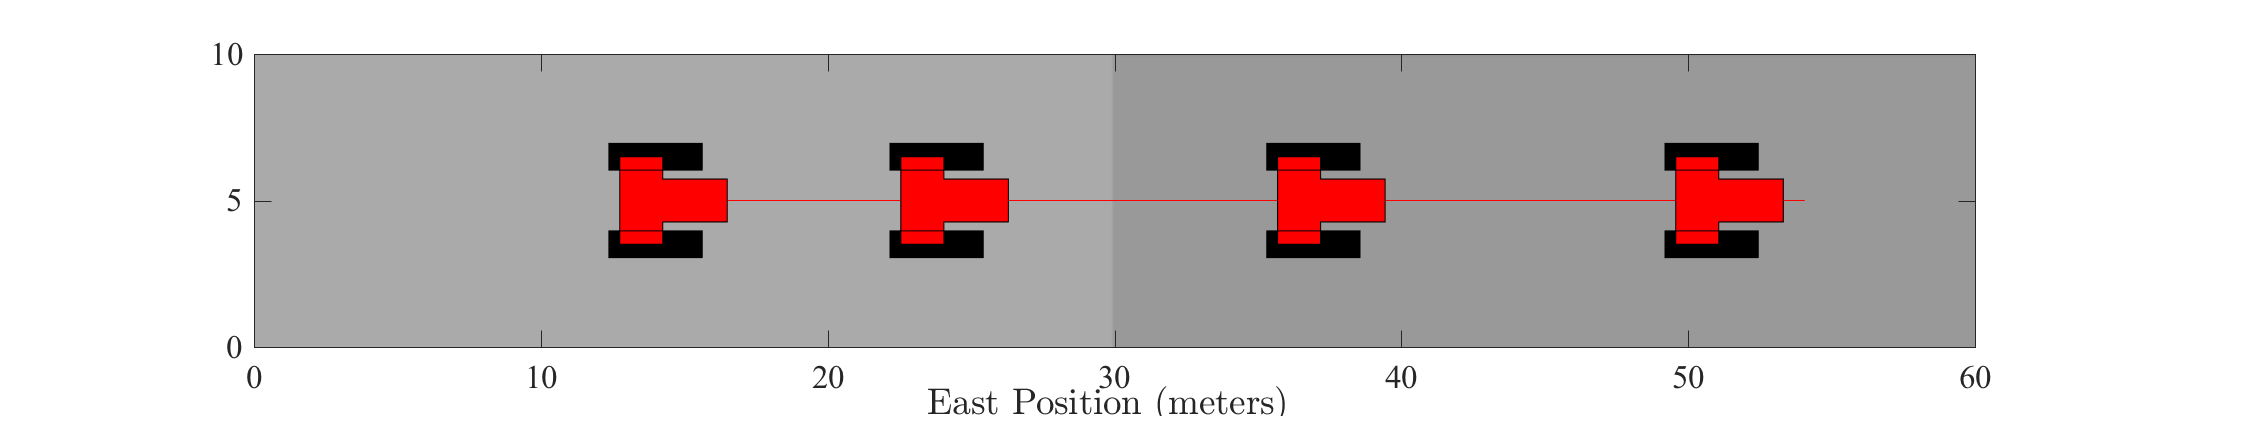
\includegraphics[width = 5.5in, keepaspectratio]{DTKF_2DPlot_1Tractor}
    \caption{1 Tractor colored red traversing two different terrains pulling an 80,000 kg payload. The starting terrain on the left is firmer and provides plenty of traction. with terrain parameters $c = 6.1\hspace{1mm}kPa$, $\Phi = 20^o$, $n = 1$, $keq = 500$, $K = 2\hspace{1mm}cm$, $S = \frac{0.6}{33}$. The second terrain is softer and the tractor becomes immobilized. The terrain paramters for this terrian are $c = 3\hspace{1mm}kPa$, $\Phi = 18.1^o$, $n = 1$, $keq = 333$, $K = 0.7\hspace{1mm}cm$, $S = \frac{0.8}{33}$.}
    \label{fig:DTKF_2DPlot_1Tractor}
\end{figure}
\begin{figure}[htb]
    \centering
    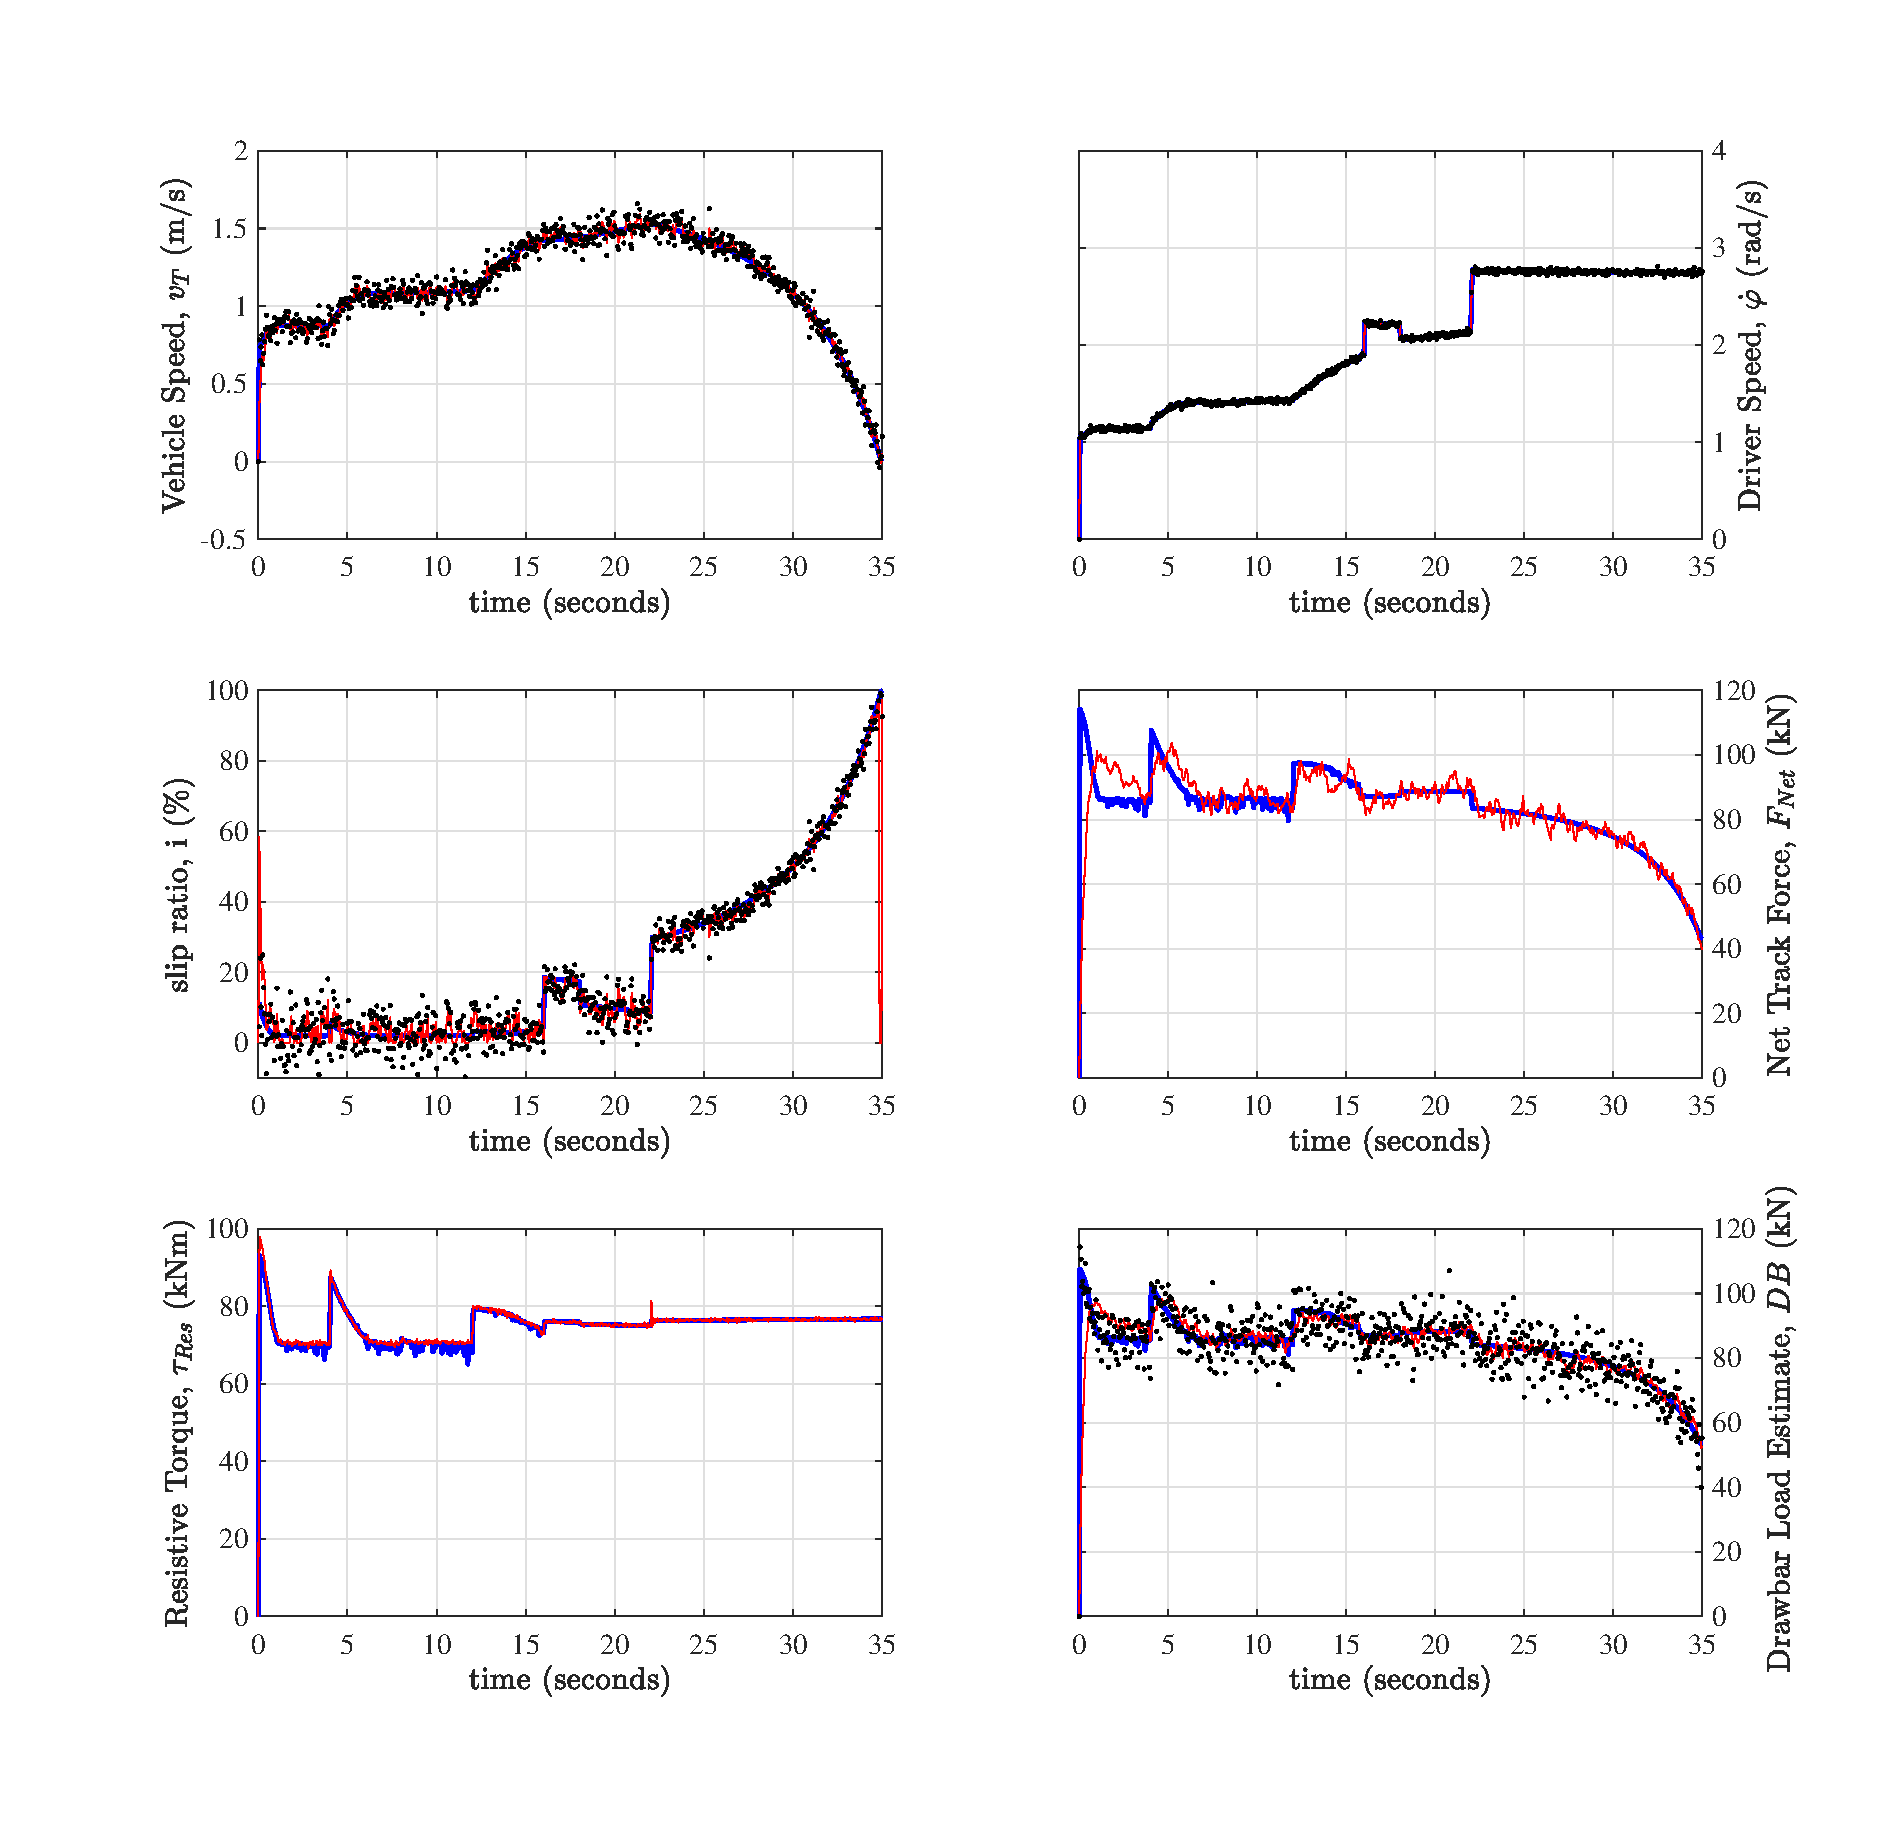
\includegraphics[width = 6in, keepaspectratio]{DTKF_Traj_1Tractor}
    \vspace{-40pt}
    \caption{Plots of tractor speed $v_T$, driver speed $\dot\varphi$, slip ratio $i$, net traction force $F_{net}$, resistive torque $\tau_{res}$, and drawbar load $DB$. Measured values are denoted as black dots, estimated values that are outputs from the DTKF are red, and true values are blue.}
    \label{fig:DTKF_Traj_1Tractor}
\end{figure}
\begin{figure}[htb]
    \centering
    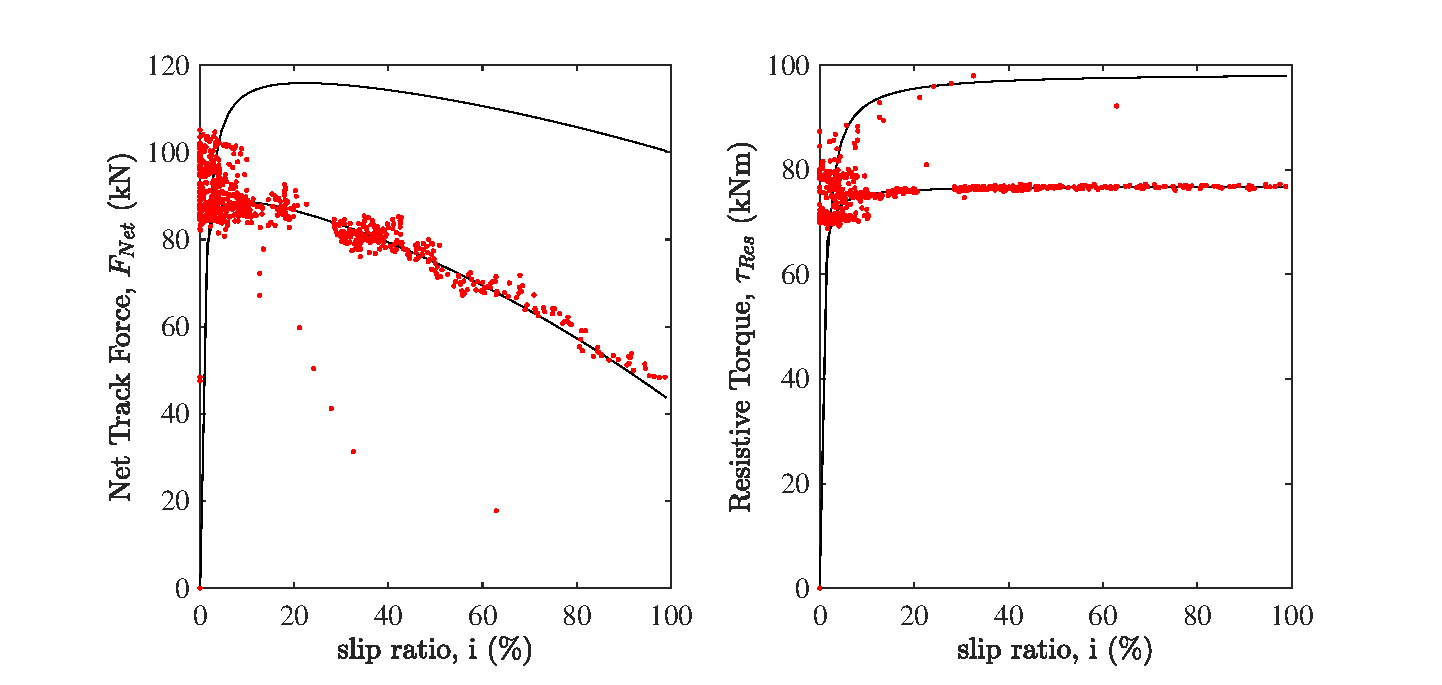
\includegraphics[height = 2.5in, keepaspectratio]{DTKF_Force_Estimates_Model}
    \caption{Net traction force curves, $F_{net}$, and resistance torque curves, $\tau_{res}$ for both the firm, starting terrain and softer terrain shown in Fig \ref{fig:DTKF_2DPlot_1Tractor}. The terrain parameters for the firm, starting terrain are $c = 6.1\hspace{1mm}kPa$, $\Phi = 20^o$, $n = 1$, $keq = 500$, $K = 2\hspace{1mm}cm$, $S = \frac{0.6}{33}$. The softer terrain has parameters of $c = 3\hspace{1mm}kPa$, $\Phi = 18.1^o$, $n = 1$, $keq = 333$, $K = 0.7\hspace{1mm}cm$, $S = \frac{0.8}{33}$.}
    \label{fig:DTKF_Force_Estimates_Model}
\end{figure}
Figure \ref{fig:DTKF_Force_Estimates_Model} plots slip, net traction estimate pairs, $[\hat{i}_k,\hat{F}_{net}]$, and slip, resistance torque pairs, $[i,\tau_{res}]$, plotted against the true curves for the two different terrains. This gives another illustration in addition to Fig. \ref{fig:DTKF_Traj_1Tractor} about the accurracy of the estimates from the DTKF. The output from the DTKF used for terrain estimation is the estimated slip $\hat{i}_k$ and the vector $\hat{\mathbf{F}}_k \equiv [\hat{F}_{net},\hat{\tau}_{res}]^T$ at each time step $k$.